		\subsection{Max flow}
			We can make nodes $v_{u,v},\{u,v\}\in E$, $v_i,i\in V$, a source $S$ and a sink $T$. Then connect edges from $S$ to $v_{u,v}$ with capacity of $1$, from $v_{u,v}$ to $v_u$ and $v_v$ with capacity of $1$ and from $v_i$ to $T$ with capacity of $c(i)$. If this graph has a maximum flow of $|E|$, then the original graph has a feasible orientation.\par
			\begin{figure}[H]
				\centering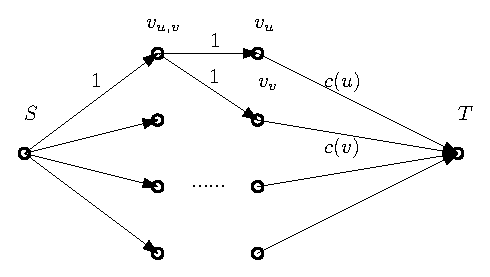
\includegraphics[width=3in]{source/qwd/qa.eps}
			\end{figure}
			For a maximum flow $S$, since the flow is full and nodes $v_{u,v}$ has exactly one unit flow input, exactly one of the edges $<v_{u,v}, v_u>$ and $<v_{u,v}, v_v>$ will has a flow. We can simply orientate edge $\{u,v\}$ to $u\to v$ if $<u_{u,v}, v_v>$ has a flow, or $v\to u$ if $<u_{u,v}, v_u>$ has a flow. Thus, the in-dgree of $i$ is just the flow through $v_i$, which is less than or equal to the capacity to sink, $c(i)$. So, we get a feasible orientation.\par
			For a feasible orientation, %since convert ${u,v}$ to both $<u,v>$ and $<v,u>$ is meaningless(otherwise we can delete one of them and make maximum in-dgree of $u$ and $v$ decreas by $1$).
			if $\{u, v\}$ is converted to $u\to v$, we can add the flow on path $S\to v_{u, v}\to v_v\to T$ by one unit, or $S\to v_{u, v}\to v_u\to T$ when converted to $v\to u$. Since the in-degree of a node $i$ doesn't exceed $c(i)$, so the flow from $v_i$ to $T$ is less than or equal to the capacity $c(i)$.
		\subsection{Maximum matching}
			We can make nodes $vl_{u,v},\{u,v\}\in E$ as $X$ and $vr_{i,j},i\in V,1\leq j\leq c(i)$ as $Y$. Then connect $c(u)$ edges between $vl_{u, v}$ and $vr_{u,j},1\leq j\leq c(u)$, $c(v)$ edges between $vl_{u, v}$ and $vr_{v,k},1\leq k\leq c(v)$. If this bipartite graph has a maximum matching of size $|E|$, then the original graph has a feasible orientation.\par
			\begin{figure}[H]
				\centering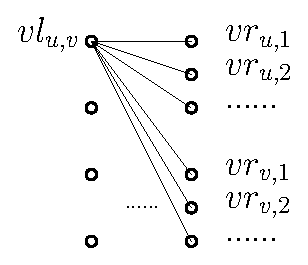
\includegraphics[width=2in]{source/qwd/qb.eps}
			\end{figure}
			For a maximum matching $S$, since the size of matching is $|E|$, every node $vl_{u, v}$ has a paired node in $Y$, then we convert $\{u, v\}$ to $u\to v$ if the paired node is $vr_{v,i}$, or to $v\to u$ if that node is $vr_{u,i}$. Since nodes $vr_{i, j}$ in $Y$ is no more than $c(i)$, so the in-degree of $i$ is less or equal to $c(i)$. Then we get a feasible orientation.\par
			For a feasible orientaion, we processe edges one by one in an arbitrary order. If $\{u, v\}$ is converted to $u\to v$, we can match $vl_{u, v}$ with $vr_{v, i}$, or $vr_{u, j}$ when converted to $v\to u$, where $i$ and $j$ is the smallest one that $vr_{v, i}$, $vr_{u, j}$ has not matched before. Since the in-degree of a node $i$ doesn't exceed $c(i)$, so there is always an avalible $i$ or $j$.